\documentclass[12pt]{article}
 \usepackage[margin=1in]{geometry}
\usepackage{amsmath,amsthm,amssymb,amsfonts}

\newcommand{\N}{\mathbb{N}}
\newcommand{\Z}{\mathbb{Z}}

\newenvironment{problem}[2][Problem]{\begin{trivlist}
\item[\hskip \labelsep {\bfseries #1}\hskip \labelsep {\bfseries #2.}]}{\end{trivlist}}
%If you want to title your bold things something different just make another thing exactly like this but replace "problem" with the name of the thing you want, like theorem or lemma or whatever


\usepackage{tkz-fct}  
\usepackage[parfill]{parskip, scrartcl}

\begin{document}

%\renewcommand{\qedsymbol}{\filledbox}
%Good resources for looking up how to do stuff:
%Binary operators: http://www.access2science.com/latex/Binary.html
%General help: http://en.wikibooks.org/wiki/LaTeX/Mathematics
%Or just google stuff

\title{Math 53: Week 1 Homework}
\author{Abhijay Bhatnagar}
\maketitle

\setcounter{secnumdepth}{0} %% no numbering
\section{Assignment}

Section 10.1: 1, 2, 3, 5, 7, 11, 12, 24, 37, 38

Section 10.2: 1, 2, 3, 4, 5, 11, 13, 17, 18, 19, 29, 30, 32, 33, 41, 42, 43, 44, 48, 51, 52, 53, 73, 74
\newline


\begin{problem}{10.1.1}
Statement of problem goes here
\end{problem}

\begin{proof}
Proof goes here. Repeat as needed
\end{proof}

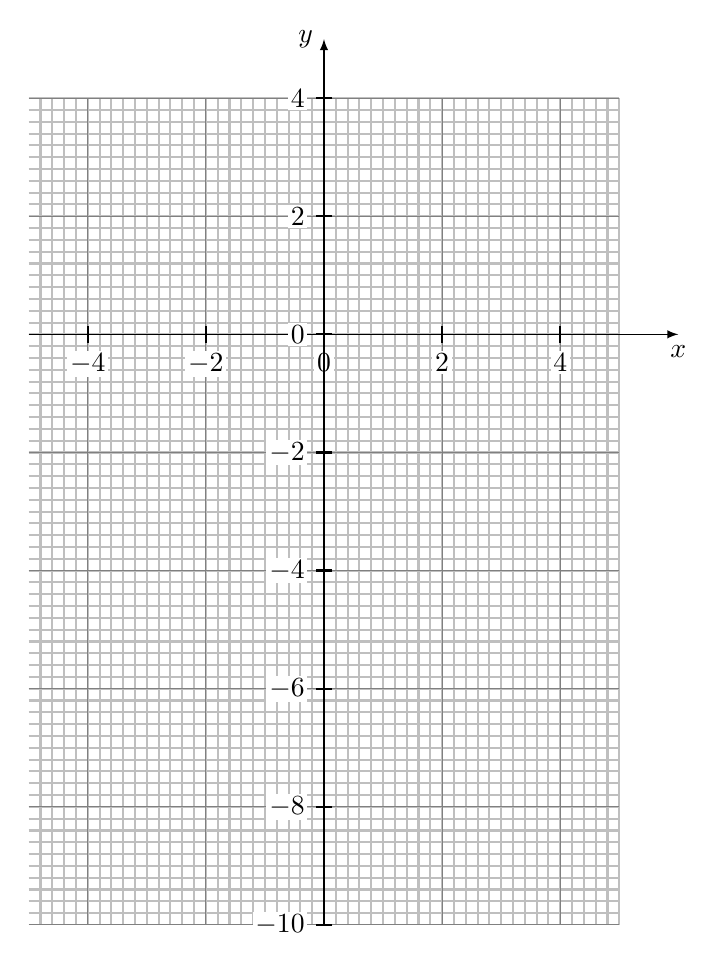
\begin{tikzpicture}[scale=1.5]
  \tkzInit[xmin=-5,xmax=5,xstep=2,ymin=-10,ymax=4,ystep=2]
  \tkzGrid[sub]
  \tkzAxeX[step=2]
  \tkzAxeY[step=2]
  \tkzFctPar[samples=400,domain=-pi:pi]{t**3-3*t}{3*t**2-9}
\end{tikzpicture}




\begin{problem}{x.yz}
Statement of problem goes here
\end{problem}

\begin{proof}
Proof goes here. Repeat as needed
\end{proof}

\end{document}